
The previous chapter introduced QRNNs and DRNNs as machine-learning based
methods to perform remote sensing retrievals. The motivation for this was to
find a practical approach to combine the expressiveness of modern, deep neural
networks with the theoretically sound handling of uncertainties of conventional
inverse-theory-based retrieval methods. To explore the validity and
practicality of the proposed methods we have tested them using idealized
scenarios and developed multiple real-world retrieval applications. This section
presents this work and summarizes the main results.

\section{Handling retrieval uncertainty with neural networks}

The first of the append papers, titled 'A neural network approach to estimating
a posteriori distributions of Bayesian retrieval problems' and published in
\citet{pfreundschuh18},} proposes the use of QRNNs for remote sensing
retrievals. The motivation for this study were the shortcomings the retrieval
methods that were available at the time of its writing. While the Bayesian
framework provides a principled way of handling the retrieval uncertainties
(see Sec.~\ref{sec:machine_learning:retrieval_problem}), these methods are
computationally complex and cannot easily be extended to include information
from neighboring pixels in the retrieval. While retrievals based on neural
networks were already common and often offered superior performance both in
terms of computational cost as well as accuracy,they neglected retrieval uncertainties.

Two experiments were performed in the study. The first one used an idealized
retrieval scenario in which samples from the posterior distribution $p(y|x)$
could be calculated using Markov Chain Monte Carlo (MCMC) methods. MCMC is
generally too slow to be used in operational processing, but its ability to
generate samples from the true posterior distribution makes it suitable to
provide a reference solution against which QRNNs and another Bayesian retrieval
method could be evaluated. A principal results from this experiment is shown
Fig.~\ref{fig:contributions:cdfs_qrnn_bmci}. The plot displays the retrieved
CDFs of the posterior distributions using QRNN and Bayesian Monte Carlo
Integration (BMCI), which is a commonly used Bayesian retrieval methods. Each
panel shows the reference CDF obtained using MCMC in the background and the CDFs
obtained using BMCI in blue, those obtained from a single QRNN using a solid red
line and those obtained from an ensemble of QRNNs using red markers. The shown
samples were chosen according to the Kolmogorov-Smirnov of the BMCI
($\text{KS}_\text{BMCI}$) and QRNN ($\text{KS}_\text{QRNN}$), which measures
the agreement between the reference and retrieved CDF, and thus show retrieval
results of varying quality from each retrieval.

The main finding from this first experiment is that the CDFs retrieved using
QRNN and BMCI agree very well with the reference CDF calculated using MCMC. This
indicates that probabilistic neural network retrievals are consistent with the
Bayesian solution of inverse problems with the a priori distribution being
represented by the training data.

\begin{figure}
  \centering
  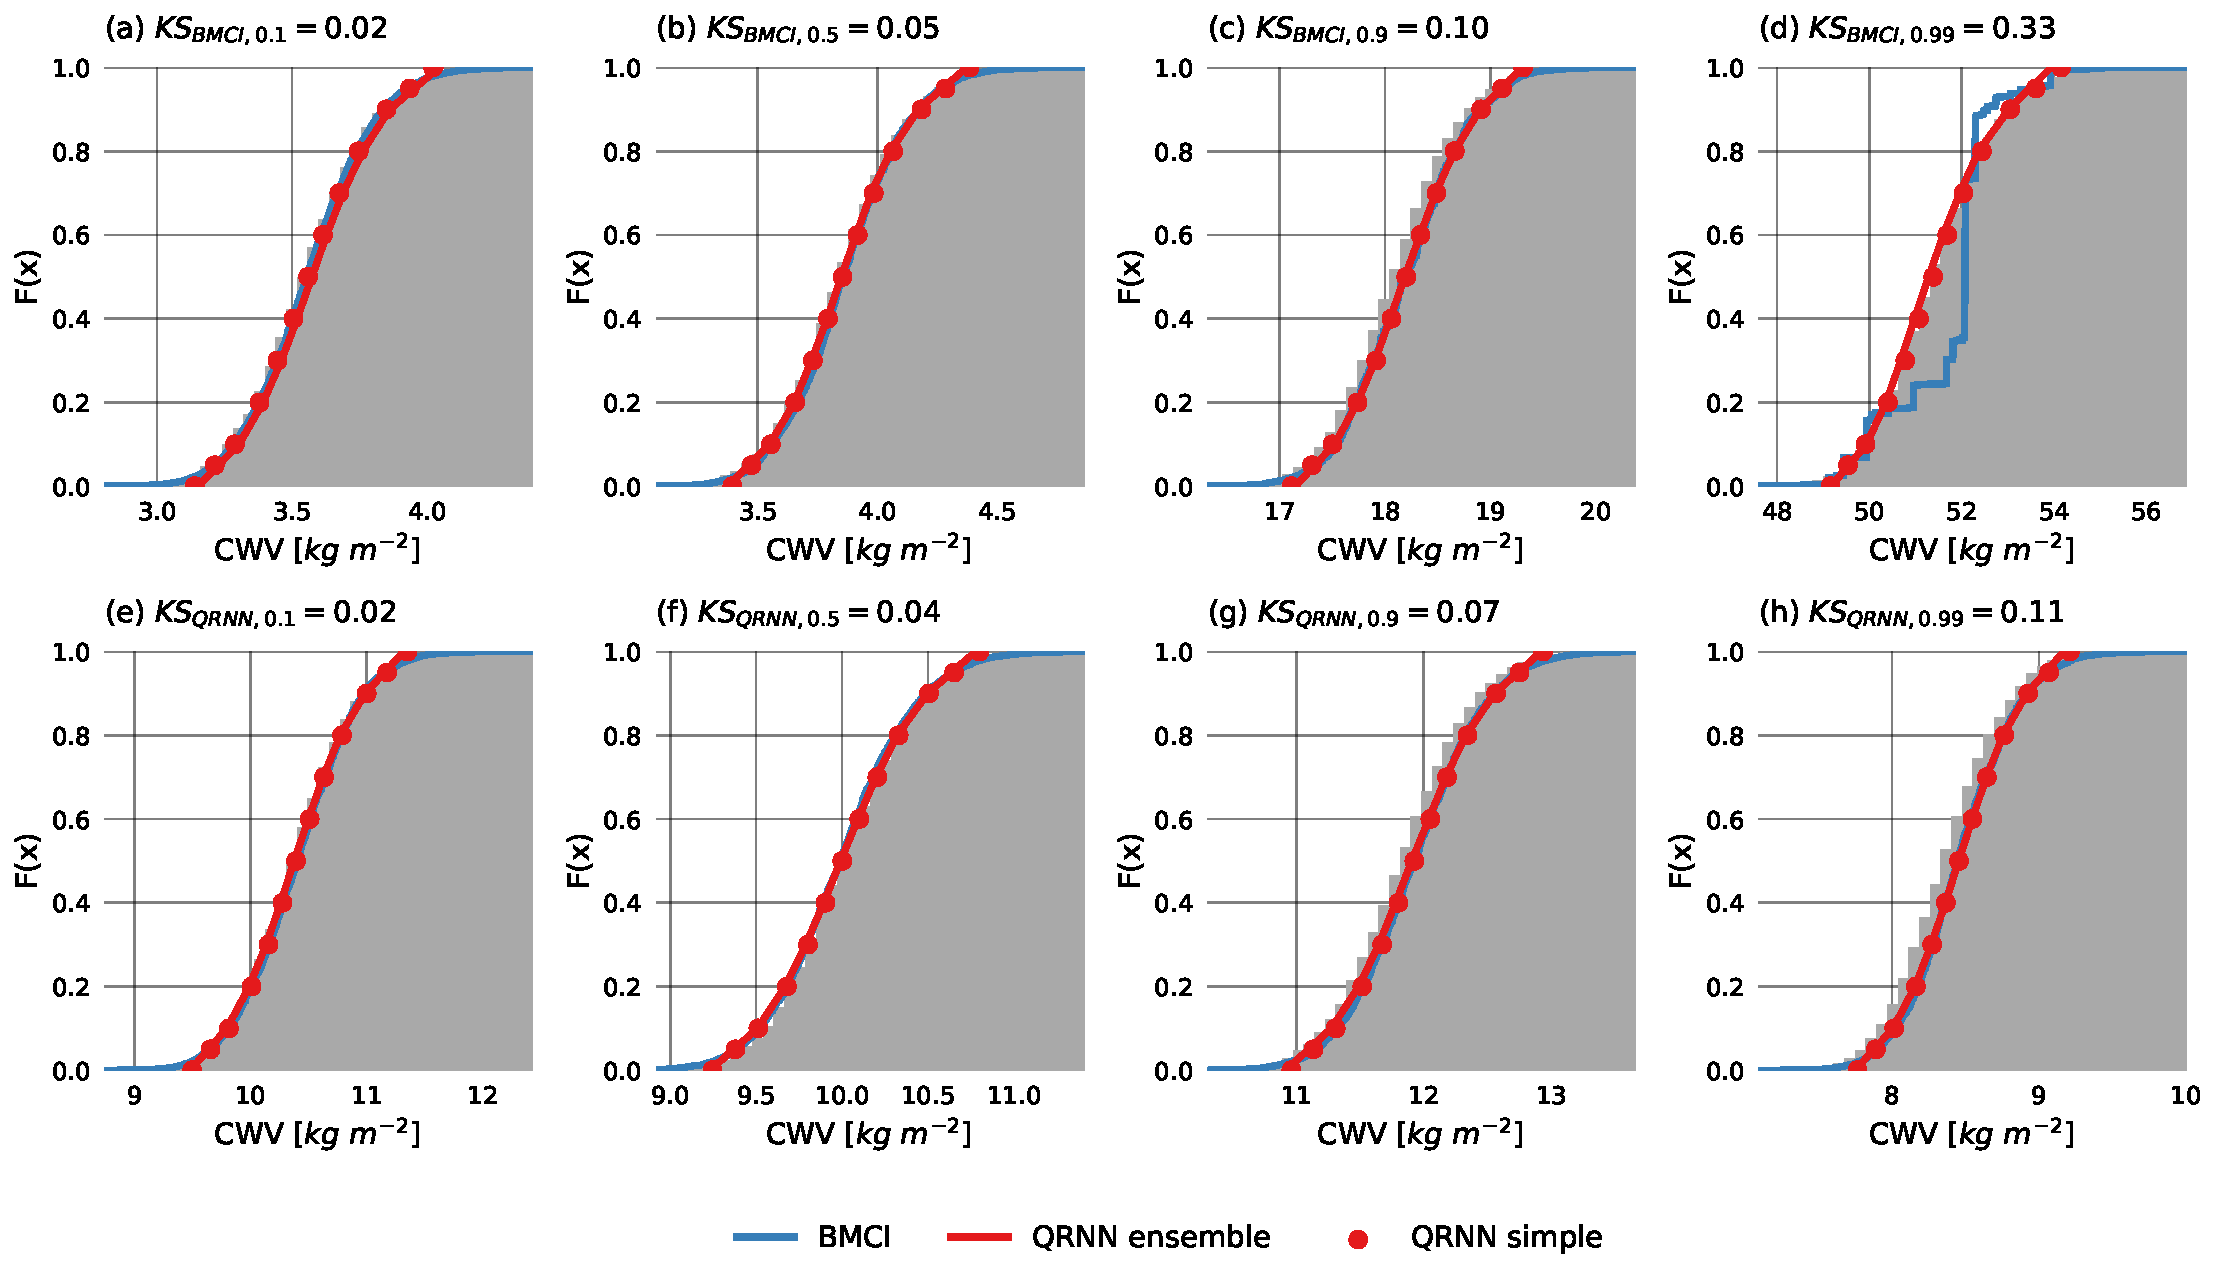
\includegraphics[width=\textwidth]{cdfs_qrnn_bmci}
  \caption{ Retrieved a posteriori CDFs obtained using MCMC (gray), BMCI (blue),
    a single QRNN (red line) and an ensemble of QRNNs (red marker). Cases
    displayed in the first row correspond to the 1st, 50th, 90th and 99th
    percentiles of the distribution of the Kolmogorov– Smirnov statistic of BMCI
    compared to the MCMC reference. The second row displays the same percentiles
    of the distribution of the Kolmogorov–Smirnov statistic of the single-QRNN
    predictions compared to MCMC.}
  \label{fig:contributions:cdfs_qrnn_bmci}
\end{figure}

The second experiment from this study applied QRNNs to the retrieval of cloud
top pressure (CTP) from infrared observations from the Moderate Resolution
Imaging Spectroradiometer (MODIS). Comparison of the QRNN retrieval to an
existing, deterministic neural network retrieval showed that QRNNs yield
comparable or better accuracy for point predictions with the added benefit of
providing reliable uncertainty estimates.

The two principal results that emerged from this study were (1) the
compatibility of probabilistic neural networks with the Bayesian formulation of
the retrieval problem and (2) the viability of the approach, which allows to
combine the superior performance of neural network retrievals with the
theoretically sound treatment of uncertainties of Bayesian retrieval methods.

\section{Passive microwave precipitation retrievals}

The second study, presented in \citet{pfreundschuh22}
(Chap.~\ref{chap:gprof_nn}), follows up the methodological development from
\citet{pfreundschuh18} by exploring the application of the developed methodology
within the operational passive microwave precipitation retrievals of the GPM
mission.  GPROF is a Bayesian retrieval based based
on the BMCI method evaluated in the previous study. It is used to retrieve
surface precipitation and forms an important component in the retrieval pipeline
of the GPM precipitation products, which can be considered to be among the most
robust precipitation products currently available.

The aims of this study were to assess the potential benefits of replacing the
currently used Bayesian retrieval method with a neural network based retrieval.
In addition to this, the study aimed to explore to what extent the retrieval
accuracy can be improved if structural information from neighboring pixels is
incorporated into the retrieval instead of process each pixel separately as the
current implementation does. To this end, two neural network based
implementation were developed. The first one, named GPROF-NN 1D, uses an MLP to
retrieve precipitation from a single pixel. The second one, GPROF-NN 3D, uses a
CNN to retrieve precipitation across the full swath simultaneously. This allows
the retrieval to leverage structural information in the observations, that is
not available to the other retrievals.

Both the GPROF-NN 1D and GPROF-NN 3D retrieval were developed to be functionally
equivalent to the currently operational GPROF algorithm so that they can
potentially replace it in an upcoming update. Moreover, the implementations were
restricted to use exactly the same data for the training as the current method
to ensure a fair comparison of the three retrievals. This required the development of
a training pipeline that can be applied to all sensors of the GPM constellation.
This proved challenging especially for the GPROF-NN 3D retrieval. The training
data for all sensors of the GPM constellation is based on combined
radar/radiometer observations from the GPM satellite. Since these observations
are only available at a $\SI{100}{\kilo \meter}$-wide swath at the center of the
GMI observations, a way had to be found to extent these to the full GMI-swath
and to remap them to the viewing geometries of the other sensors. The current
approach uses an intermediate simulator network to extend the simulated
observations to the full swath of GMI, which are then remapped to the viewing
geometries of other sensors by interpolation. This solution should be a
considered a heuristic that was pursued mainly because extending the simulations
that are routinely performed for the generation of the GPROF training data would
have been outside the scope of this study.

The main results from this study are estimates of potential improvements in
retrieval accuracy that can be realized by upgrading GPROF to either the
GPROF-NN 1D or GPROF-NN 3D retrieval. To isolate the effect of the retrieval
method from the actual training data, the retrieval accuracy was assessed using
held-out scenes from the training data. We found consistent improvements for the
GPROF-NN 1D algorithms across a range of accuracy metrics and across all
retrieved quantities. The accuracy can be improved further by switching to the
GPROF-NN 3D retrieval, which yields additional improvements similar in magnitude
to those provided by the GPROF-NN 1D algorithm of the GPROF baseline retrieval.
Moreover, we found that the effective resolution of the retrieval improves by at
least $\SI{40}{\percent}$ with the neural network based retrieval. The study
included results from two case studies of Hurricane overpasses from the GMI and
MHS sensors, which provided limited evidence that the retrieval improvements can
be expected to carry over to real observations.

While the results from \citet{pfreundschuh22} were promising, their significance
was limited due to the evaluation being mostly based on observations from the
same distribution as the training data. Since for GMI the training data
consisted of real observations, these results can be expected to carry over to
operational application of the retrieval. For the other sensors, however, this
is less evident because their training consists of simulated observations whose
distribution deviates from that of real observations. In addition to this, the
question remained open to what extent the retrieval results that are closer to
the training data actually improve precipitation estimates compared to
independent validation data.

The study presented \citet{pfreundschuh22c} addresses these outstanding
questions. To validate the newly developed implementation of GPROF, the results
from the conventional and neural-network-based versions against ground-radar
measurements over the continental united states (CONUS) and the tropical
Pacific. The study was designed to provide a comprehensive assessment of the
errors of the GPROF retrievals in order to determine the improvements afforded
by neural-network based retrieval and to identify potential outstanding issues
impeding their adaptation to operational processing.

The validation against the ground based radar measurements largely confirmed the
results from \citet{pfreundschuh22}. Both neural-network-based retrievals
achieve significant improvements in retrieval accuracy compared to the
conventional implementation. This is also the for the effective resolution of
the retrievals, which are improved from $60$ to $\SI{20}{\kilo \meter}$ over
land surfaces and from $20$ to $\SI{15}{\kilo \meter}$ over Ocean.

\section{VIS/IR precipitation retrievals}

While the neural-network-based implementation of GPROF provided clear evidence
for the potential of neural-network based precipitation retrievals, the
constraint of a retrieval that provides the same output as the currently
operational GPROF algorithm limited the exploration of retrieval improvements to
currently available retrieval outputs. The assessments presented in
\citet{pfreundschuh22} and \citet{pfreundschuh22c} therefore focused mostly on
deterministic precipitation estimates and thus did not explore the full
potential of the probabilistic predictions afforded by the neural network.

The aim of the study presented in \citet{pfreundschuh22b} was to explore the
full potential of probabilistic neural-network based precipitation retrievals in
the context of near real-time retrievals from VIS/IR observations over Brazil.
The input data for the retrieval comes from the advanced baseline imager (ABI)
on the geostationary operational environmental satellite (GOES) 16. To train the
retrieval, the input observation were co-located with combined radar-radiometer
measurements from the GPM core observatory satellite.

To validate the retrieval its results were compared to 1 month of gauge
measurements. The retrieval accuracy was assessed by comparing it to the
retrieval algorithm that is currently used operationally at the Brazilian
institute of space research as well as to commonly used global precipitation
retrievals. We were able to show that, despite the limited information content
of VIS/IR observations, deep-learning-based retrievals outperform currently
available methods, even those that merge IR observations from geostationary
satellite with PMW observations polar-orbiting platforms.

Furthermore, the study explored the potential of the probabilistic precipitation
estimates. We were able to show that, after correcting for differences in the
precipitation statistics of the training data and gauge measurements, confidence
intervals derived from the probabilistic predictions were well calibrated
against the gauge measurements. We also provided results that the probabilistic
predictions improve the detection of heavy precipitation.


\section{Cloud correction for data assimilation}

The final study included in this thesis explores the application of QRNNs to
remove the effect of clouds from microwave observations. The observations
contain important information on the distribution water vapor in the atmosphere
and are used in data assimilation systems to find good initial conditions for
numerical weather forecasts. However, the presence of hydrometeors in the
atmosphere makes radiative transfer calculation much more complex which
complicates the use of observations. Since the information on the hydrometeors
themselves is not really used in the data assimilation system, a model that
could accurately predict how these observations would look when the effect of
the hydrometeors was removed, would allow these observations to in a less
complex and computationally more efficient way.

Because of their impact on the radiative transfer, operational data assimilation
systems have to detect observations that are affected by clouds to either
correctly handle them if the DA system is sufficiently advanced to handle cloudy
observations or to discard them altogether. The first experiment therefore
assessed the potential of applying QRNN to correct cloud-contaminated
observations from an existing sensor and compared the performance to existing
methods. The experiment showed that the QRNN-derived correction leads to a lower
bias in the observations than the residual biases in currently used filtering
methods, which reject up to $\SI{30}{\percent}$. The important point here is that the QRNN-based
cloud correction achieves this without rejecting any observations, which would
makes more observations available to the data assimilation system.

The second experiment then extended the approach to a soon-to-be-launched and
and a hypothetical satellite sensor. Both of the will carry microwave sensors
with channels above $\SI{300}{\giga \hertz}$. These high frequencies make the
observations more sensible to scattering from ice particles, which further
complicates their use in data assimilation. In these cases QRNN-based cloud
correction would provide a simple alternative to ingesting this information into
data assimilation systems by using the hydrometeor information afforded by the
high-frequency channels to improve the removal of cloud contamination at lower
frequency channels. The results show that channels at frequencies exceeding
$\SI{300}{\giga \hertz}$ are well suited for cloud correction.

This study proposed a novel application of QRNNs for the correction of microwave
observations for use in data assimilation and retrievals of water vapor
profiles. QRNN-based cloud correction provides superior performance to existing
methods. In addition to that, the predicted uncertainties provide more accurate
error estimates than currently used error models for data assimilation.
Finally, the simulation-based assessment of the potential of microwave observations
at sub-millimeter wavelength lead to the selection of these channels for an
upcoming satellite mission \citep{arctic_weather_satellite}.

\section{Future work}

The findings of this thesis suggests several directions of future research.
These will be discussed below.

\subsection{Handling retrieval uncertainty with neural networks}

This thesis has proposed and assessed to neural-network-based methods for
handling uncertainties in remote sensing retrievals and shown their practicality
across multiple retrieval applications. The advantage of these methods is
certainly their simplicity. Only a minor modification in the training process is
required to migrate a deterministic neural network retrieval to a probabilistic
one.

There are, however, two important limitations of the approaches: Their
incapability of handling correlations in the retrieval outputs and their
reliance on the aleatoric assumption, which postulates that the predictive
uncertainty is dominated by the aleatoric uncertainty.

It would therefore be valuable to systematically evaluate the approaches against
Bayesian neural networks and generative model on a set of atmospheric retrieval
problems. In particular, it would be important to evaluate the methods not only
with respect to retrieval accuracy but to also take into account the effect on
downstream applications of the data. This would provide guidance in what scenarios
the computationally more complex alternative approaches should be applied.

\subsection{GPM precipitation retrievals}

Due to the good performance of the developed GPROF-NN retrievals, they are being
considered for operational implementation for the PMW precipitation retrieval of
the GPM mission. This will require some additional investigations regarding the
climatological stability of the GPROF-NN retrievals across different satellites.

In addition to that, the migration to a neural-network-based implementation
opens up for a number of improvements of the GPROF retrieval. One of them is the
extension of the training data to cover multiple years of observations. As was
found in \citep{pfreundschuh22c}, this may improve the climatic stability of the
retrieval. Furthermore, including samples from the posterior distribution may
improve the representation of extreme precipitation in the retrieval results,
which is relevant for climatological studies.

\subsection{VIS/IR precipitation retrievals}

The results presented in \citet{pfreundschuh22b} clearly showed the
potential of deep neural networks for precipitation retrieval from
geostationary satellites. According to personal communication, the
developed retrieval is also considered for operational application.

An interesting result that emerged from this study was that, despite the low
information content of the geostationary observations on precipitation,
deep-learning-based retrievals can outperform highly complex retrieval pipelines
which integrate observations from multiple sensors. This indicates that the use
of information in multi-sensor retrievals is sub-optimal. In a future project,
we will therefore explore the potential of fusing observations from different
sensors directly using a single neural network.
